\section{Additional Information for Model Testing}
\label{sec:outreach}

Other models of new physics in the dilepton final state can be confronted in an approximate way by simple 
generator-level studies that compare the expected number of events in \lumi~
with our upper limits of \ulloose~events (loose signal region) and \ultight~events 
(tight signal regions).  
The key ingredients of such studies are the kinematic cuts described 
in this note, the lepton efficiencies, and the detector response for MET.

%{\bf In the following, I am using ttbar as a `baseline' to quote ID/iso efficiencies.
%\bf Should I instead use, for example, Z+$\geq$2 jet events?}
The muon identification efficiency is $\approx 91\%$;
the electron identification efficiency varies appriximately linearly 
from $\approx$ 85\% at 
$P_T = 20$~GeV to 93\% for $P_T > 60$~GeV (see Fig.~\ref{fig:effttbar} top).

The lepton isolation efficiency varies with lepton momentum, as well as the jet activity in the event.
In $t\bar{t}$ events, it varies appriximately linearly from $\approx 85\%$ (muons)
and $\approx 88\%$ (electrons) at $P_T=20$~GeV to $\approx 97\%$ for $P_T>60$~GeV. 
In LM4 (LM8) events, this efficiency is degraded by $\approx 5$\% ($\approx 10$\%) over the whole momentum 
spectrum (see Fig.~\ref{fig:effttbar} bottom).

The average detector response (the reconstructed quantity normalized to the generated quantity) 
for MET is 
consistent with unity within the 5\% jet energy scale uncertainty.
%$0.96 \pm X$ where the uncertainties originate from the hadronic energy scale uncertainty.
The experimental resolution on this quantity is 12\%. See figure \ref{fig:LM4_met}.


\begin{figure}[tbh]
\begin{center}
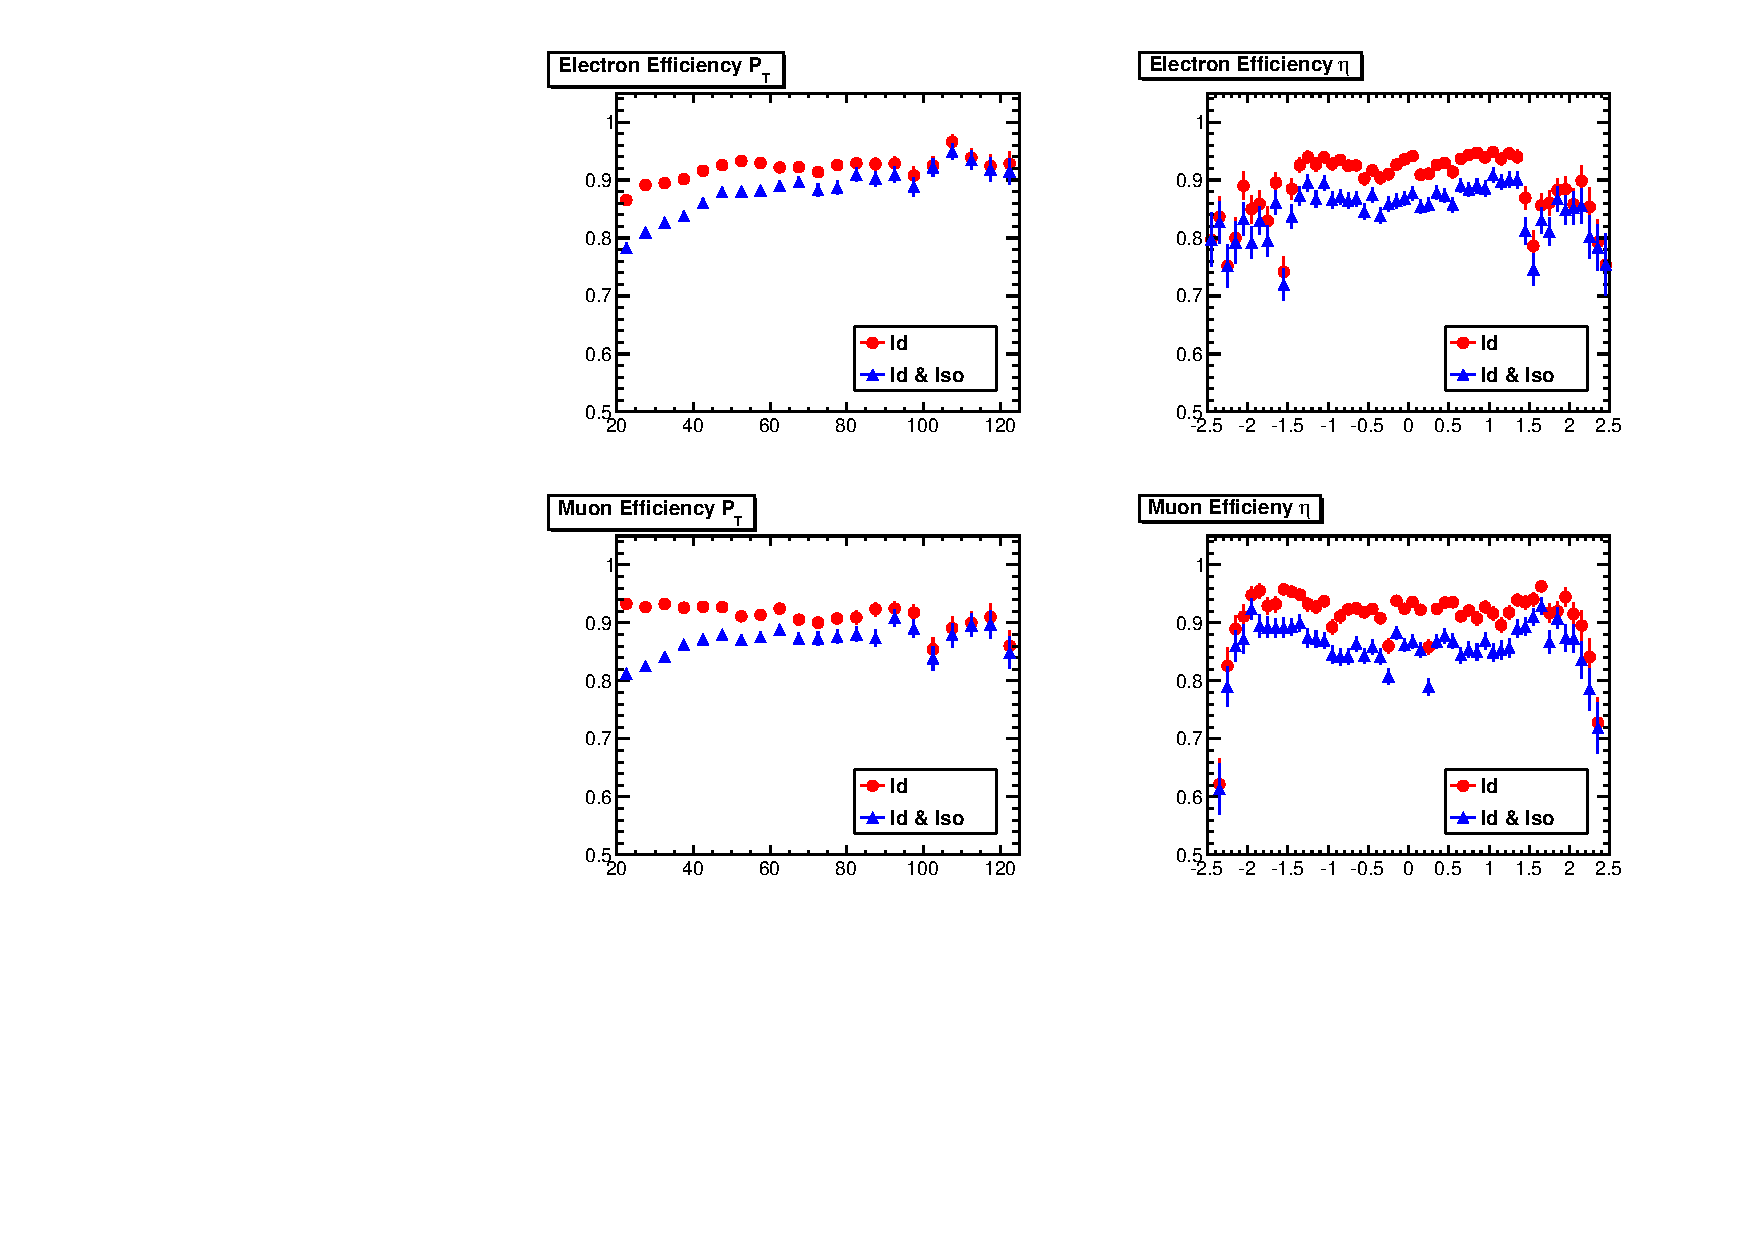
\includegraphics[width=1.0\linewidth]{plots/ttbar_eff.pdf}
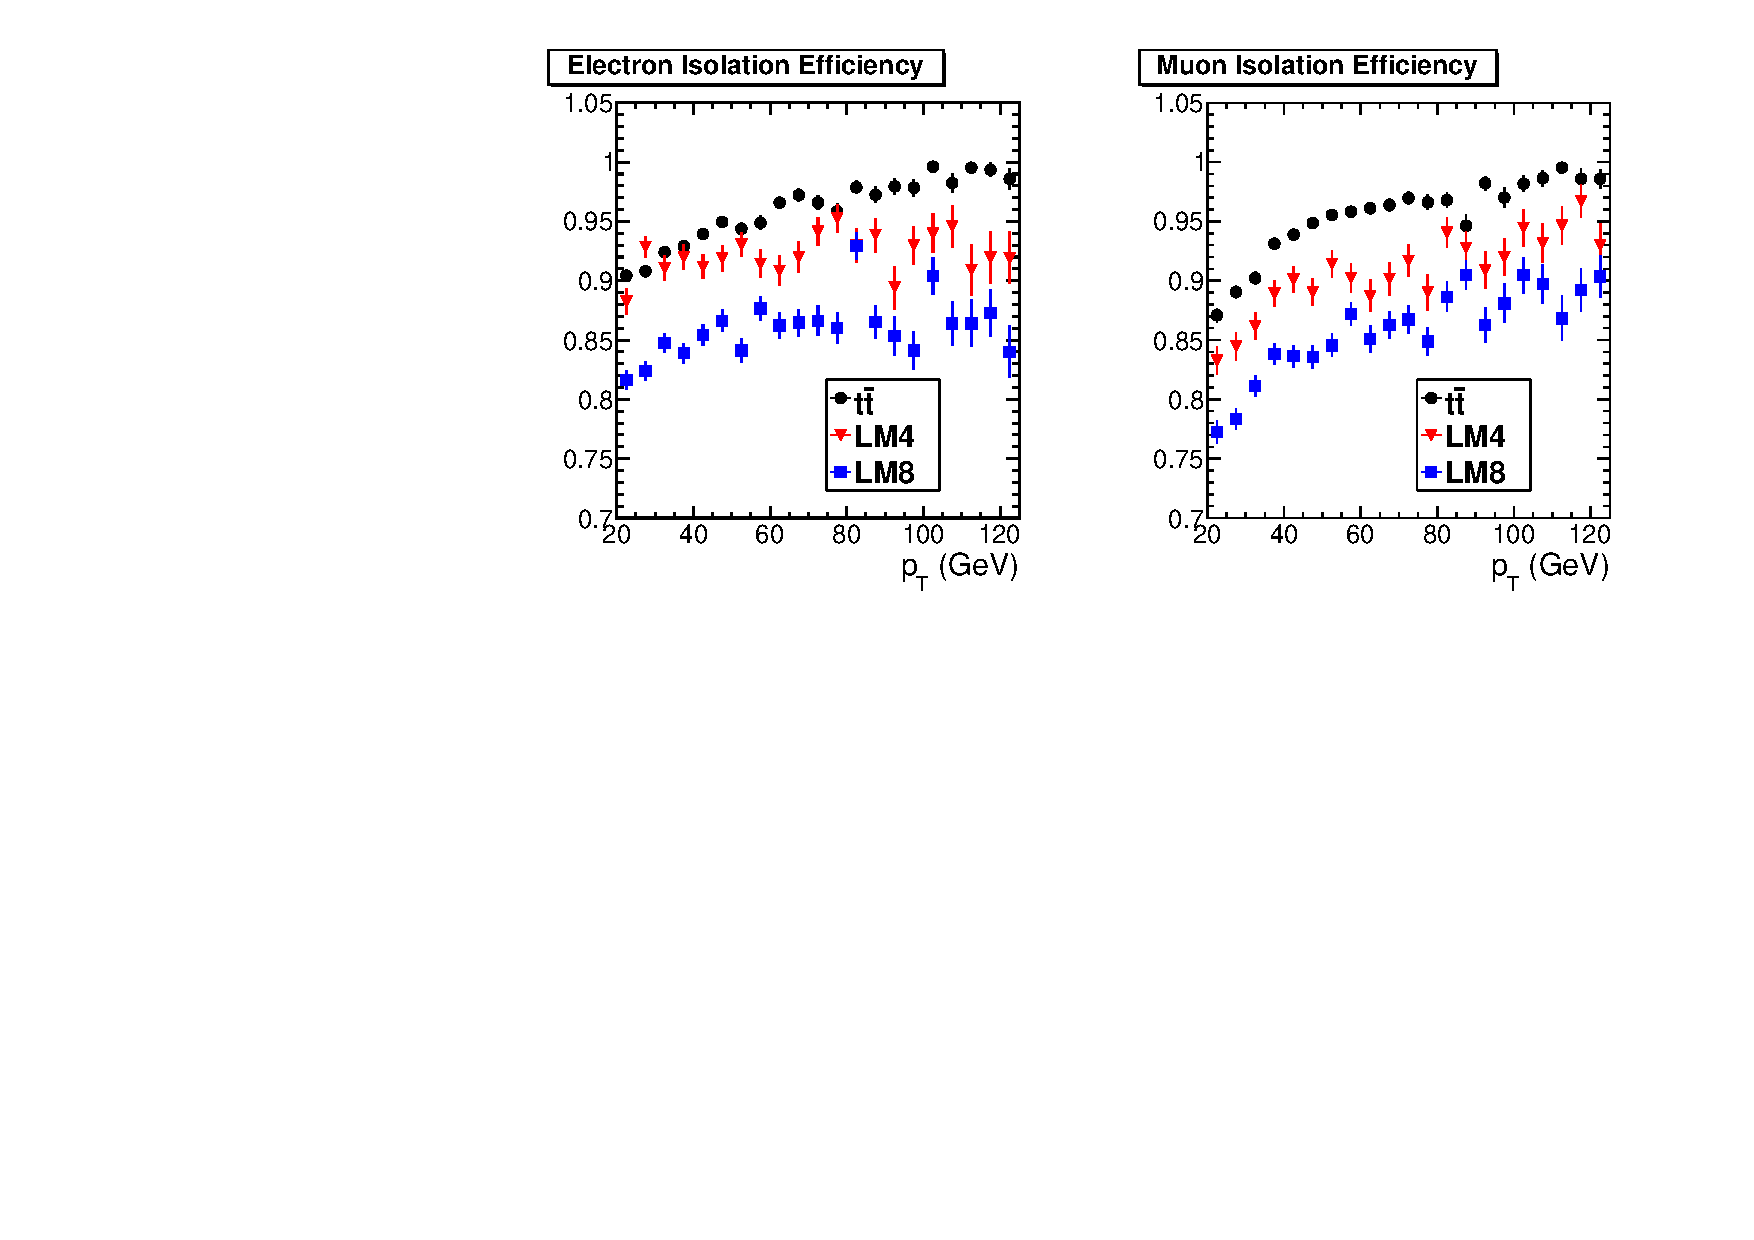
\includegraphics[width=1.0\linewidth]{plots/ttbar_LM4_LM8_isoeff.pdf}
\caption{\label{fig:effttbar}\protect 
Identification and isolation efficiencies for leptons from $t \to W \to \ell$ and 
$t \to W \to \tau \to \ell$ in $t\bar{t}$ events (top). Isolation efficiency
for $t\bar{t}$, LM4 and LM8 (bottom).}
\end{center}
\end{figure}

\begin{figure}[tbh]
  \begin{center}
	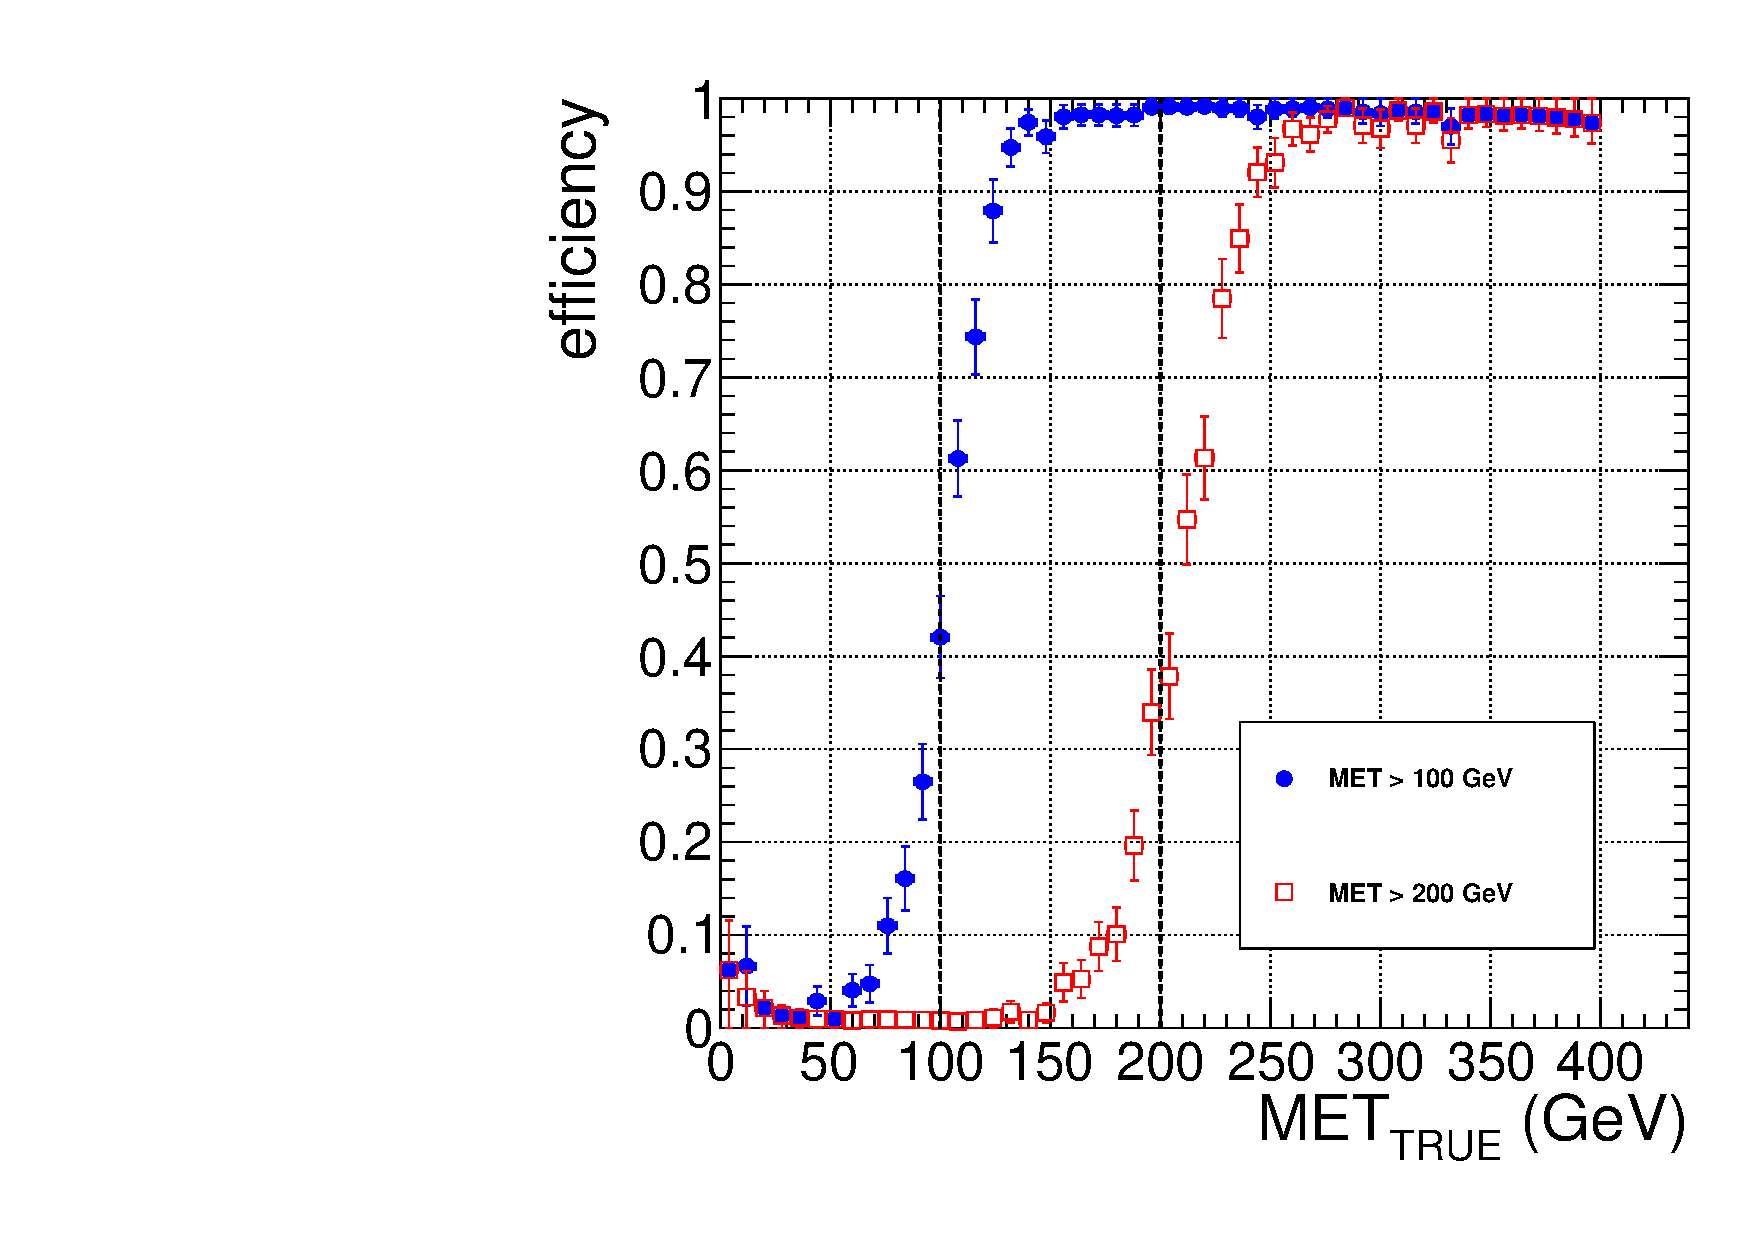
\includegraphics[width=0.45\linewidth]{plots/met_efficiency.pdf}
	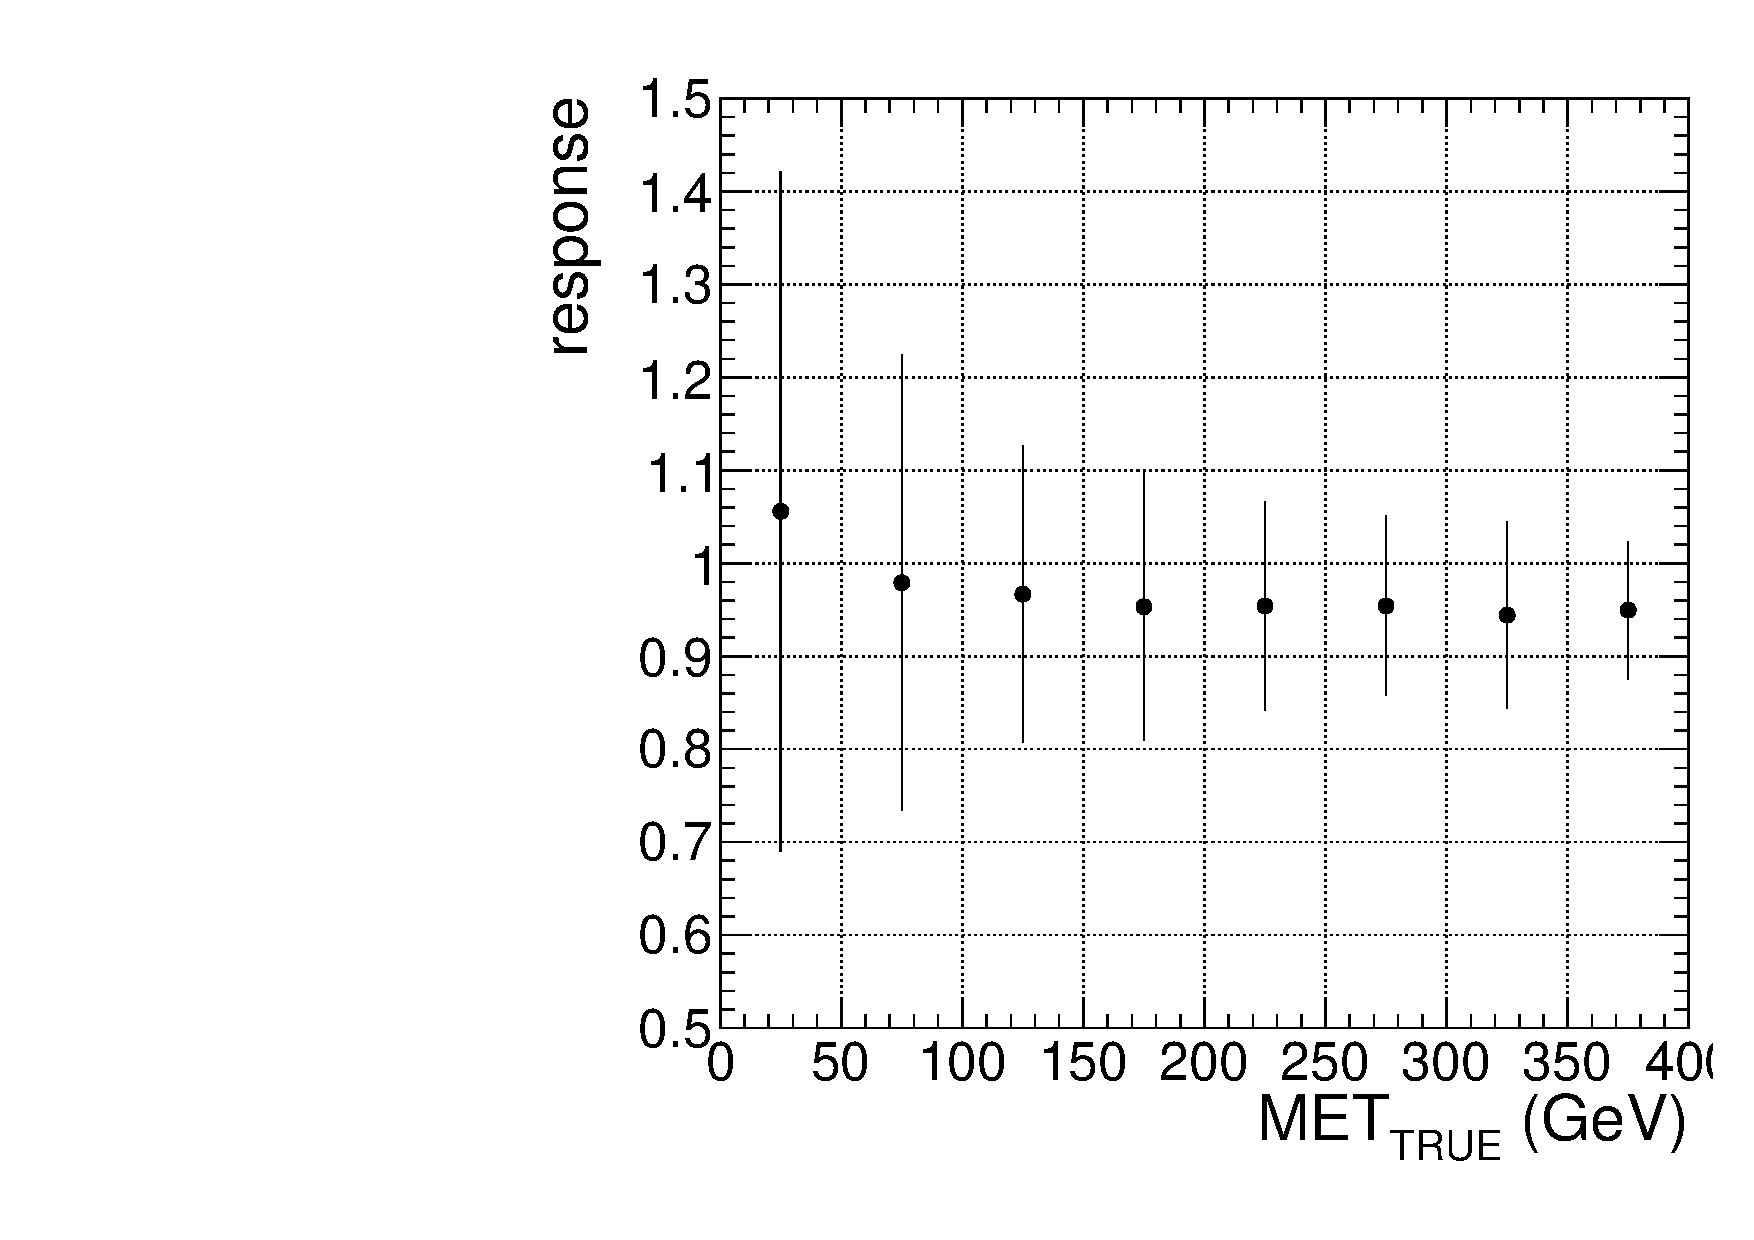
\includegraphics[width=0.45\linewidth]{plots/met_response.pdf}
	\caption{\label{fig:LM4_met}\protect 
	  Left: the efficiency to pass the MET $>$ 100, 200 GeV requirements 
	  (indicated by the vertical dashed lines)
	  as a function of the true MET. Right: the average detector response
	  (reconstructed MET divided by true MET) 
	  and its RMS, as a function of true MET. These plots are made with LM4 MC, but they are 
	  not expected to depend
	  strongly on the underlying physics.}
  \end{center}
\end{figure}